% This is based on "sig-alternate.tex" V1.9 April 2009
% This file should be compiled with V2.4 of "sig-alternate.cls" April 2009
%
\documentclass{report}

\usepackage[english]{babel}
\usepackage{graphicx}
\usepackage{tabularx}
\usepackage{subfigure}
\usepackage{enumitem}
\usepackage{url}
\usepackage[utf8]{inputenc}
\usepackage{textcomp} %for the degree symbol. yes. overkill

\usepackage{color}
\definecolor{orange}{rgb}{1,0.5,0}
\definecolor{lightgray}{rgb}{.9,.9,.9}
\definecolor{java_keyword}{rgb}{0.37, 0.08, 0.25}
\definecolor{java_string}{rgb}{0.06, 0.10, 0.98}
\definecolor{java_comment}{rgb}{0.12, 0.38, 0.18}
\definecolor{java_doc}{rgb}{0.25,0.35,0.75}

% code listings
% code listings
\usepackage{listings}
\lstnewenvironment{Java}
  {\lstset{ language=Java,
	basicstyle=\scriptsize\ttfamily,
	backgroundcolor=\color{lightgray},
	keywordstyle=\color{java_keyword}\bfseries,
	stringstyle=\color{java_string},
	commentstyle=\color{java_comment},
	morecomment=[s][\color{java_doc}]{/**}{*/},
	tabsize=2,
	showtabs=false,
	extendedchars=true,
	showstringspaces=false,
	showspaces=false,
	breaklines=true,
	numbers=left,
	numberstyle=\tiny,
	numbersep=6pt,
	xleftmargin=3pt,
	xrightmargin=3pt,
	framexleftmargin=3pt,
	framexrightmargin=3pt,
	captionpos=b
  }
  }
  {}
\lstnewenvironment{XML}
  {\lstset{language=XML}}
  {}	

\lstdefinelanguage{XML}
{
  morestring=[b]",
  morestring=[s]{>}{<},
  morecomment=[s]{<?}{?>},
  stringstyle=\color{black},
  identifierstyle=\color{blue},
  keywordstyle=\color{cyan},
  morekeywords={xmlns,version,type}% list your attributes here
  basicstyle=\scriptsize\ttfamily,
	backgroundcolor=\color{lightgray},
	tabsize=2,
	showtabs=false,
	extendedchars=true,
	showstringspaces=false,
	showspaces=false,
	breaklines=true,
	numbers=left,
	numberstyle=\tiny,
	numbersep=6pt,
	xleftmargin=3pt,
	xrightmargin=3pt,
	framexleftmargin=3pt,
	framexrightmargin=3pt,
	captionpos=b
}

% Disable single lines at the start of a paragraph (Schusterjungen)

\clubpenalty = 10000

% Disable single lines at the end of a paragraph (Hurenkinder)

\widowpenalty = 10000
\displaywidowpenalty = 10000
 
% allows for colored, easy-to-find todos

\newcommand{\todo}[1]{\textsf{\textbf{\textcolor{orange}{[[#1]]}}}}

% consistent references: use these instead of \label and \ref

\newcommand{\lsec}[1]{\label{sec:#1}}
\newcommand{\lssec}[1]{\label{ssec:#1}}
\newcommand{\lfig}[1]{\label{fig:#1}}
\newcommand{\ltab}[1]{\label{tab:#1}}
\newcommand{\rsec}[1]{Section~\ref{sec:#1}}
\newcommand{\rssec}[1]{Section~\ref{ssec:#1}}
\newcommand{\rfig}[1]{Figure~\ref{fig:#1}}
\newcommand{\rtab}[1]{Table~\ref{tab:#1}}
\newcommand{\rlst}[1]{Listing~\ref{#1}}

% General information

\title{Distributed Systems -- Final Project}

% Use the \alignauthor commands to handle the names
% and affiliations for an 'aesthetic maximum' of six authors.

\numberofauthors{3} %  in this sample file, there are a *total*
% of EIGHT authors. SIX appear on the 'first-page' (for formatting
% reasons) and the remaining two appear in the \additionalauthors section.
%
\author{
% You can go ahead and credit any number of authors here,
% e.g. one 'row of three' or two rows (consisting of one row of three
% and a second row of one, two or three).
%
% The command \alignauthor (no curly braces needed) should
% precede each author name, affiliation/snail-mail address and
% e-mail address. Additionally, tag each line of
% affiliation/address with \affaddr, and tag the
% e-mail address with \email.
%
% 1st. author
\alignauthor Lukas Häfliger\\
	\affaddr{ETH ID 11-916-376}\\
	\email{haelukas@student.ethz.ch}
% 2nd. author
\alignauthor Alexandra Maximova\\
 	\affaddr{ETH ID 09-913-534}\\
 	\email{amaximov@student.ethz.ch}
%% 3rd. author
 	\alignauthor Thomas Müller\\
 	\affaddr{ETH ID 11-946-936}\\
 	\email{muelltho@student.ethz.ch} 
\and  % use '\and' if you need 'another row' of author names	
%% 4th. author
\alignauthor Christian Vonrüti\\
 	\affaddr{ETH ID 11-930-914}\\
 	\email{cvonruet@student.ethz.ch} 
%% 5th. author
\alignauthor Alexander Viand\\
	\affaddr{ETH ID 09-940-131}\\
	\email{vianda@student.ethz.ch}
%% 6th. author
\alignauthor Marko Živković\\
	\affaddr{ETH ID 10-921-211}\\
	\email{markoz@student.ethz.ch}
}


\begin{document}

\maketitle

\begin{abstract}
We present a cross-platform game that allows up to eight players (who can be using different platforms)to play together via local network, 
or alternatively allows singleplayer matches against AI opponents.
>> The game is inspired by the "light cycle" scene from the 1982 film "Tron". <<
>> The game is implemented using the Unity Engine, which is a high-level framework for game development << 
The game supports Windows x86/x86\_64 and Android with potential for easy ports to others platforms thanks to the cross platform capabilities of the Unity engine.

\end{abstract}

\section{Introduction + Prior Work}

We were inspired to create this game after playing Armagetron Advanced, an open source game that is itself inspired by the light cycle scene from Tron. 
In section <<2 we will look at Armagetron Advanced and other games inspired by "Tron" <<and android ports>>.
In section <<3, we will explain the gameplay and game mechanics that we decided to implement for our game, and in  section <<4 we will introduce Unity with a focus on its networking concepts. In section <<5 we will show how we use these concepts in our game in order to ensure <<what??>>.
In section <<6 we show our implementation of collision detection and prediction, ensuring reasonable behaviour in case of network delays that are "long" in comparison to the high in-game speeds.
In section <<7 we introduce the AI that we use in the singleplayer mode as well as our own extension to the game,  randomly roaming obstacles.
In the last section, we will give our conclusions on our game working both with Unity as well as with a larger group.

 
\section{Existing "Tron"-like games}

Armagetron Advanced is one of two open source projects that try to recreate the light cycle scene, the other being GLTron by Andreas Umbach.
GLTron is a more faithful reproduction both visually as well in terms of game mechanics of the original light cycle scene from the 1982 film while Armagetron Advanced is further removed from the original visually and offers a wide variety of gamemodes that go far beyond what is seen in the film as well as heavy customization, with parameters like base speed, arena size, number of players, etc.
We were aiming more to recreate the enjoyment of playing Armagetron Advanced rather than to be faithful to the original scene.
Since the scope of this project was very limited, we do not offer the extensive options and choice of game mode that Armagetron Advanced does, 
but rather focused on implementing the "core" game mode with fixed parameters. 
Our game is visually very dissimilar to both the original scene as well as both games. Instead, we were inspired by the aesthetics from the 2010 film "Tron Legacy" which also features a light cycle scene, which does not, however, in terms of "game mechanics", bear much resemblance to the original. >>un-nest last sntc<<

\subsection{Existing mobile solutions}
Armagetron Advanced itself is available for Windows, Linux and Mac OS but does not have an Android (or other mobile platform) port.
Armagetron Advanced offers local (split-screen), local network and internet multiplayer for up to >>????<< players. 
 There exists an android game called Androgetron developed by a member of the Armagetron Advanced community, however this is a much simplified clone  which features only split-screen multiplayer. On the official Google Play Store >>TM!!<< there are a few more games >>list??<< that are essentially identical to Androgetron and seem to be all based on an android port of GLTron. They also do not offer any kind of non-split-screen multiplayer.

Split screen is a viable option on a full size laptop or desktop monitor, however it feels very cramped even on larger tablets and is essentially unusable on smartphones.
Our goal was therefore to implement a true (networked) multiplayer experience on mobile devices.
Instead of trying to adapt the large and complex code base of Armagetron Advanced (or GLTron), we decided to implement a version of the game with smaller scope from scratch.
>>Mention OpenGL being waaay too complex?<<
We decided to use Unity, a high level game engine and Integrated Development Engine (IDE) (which will be discussed in section 3), to implement the following game mechanics:

\begin{figure}
 	 	    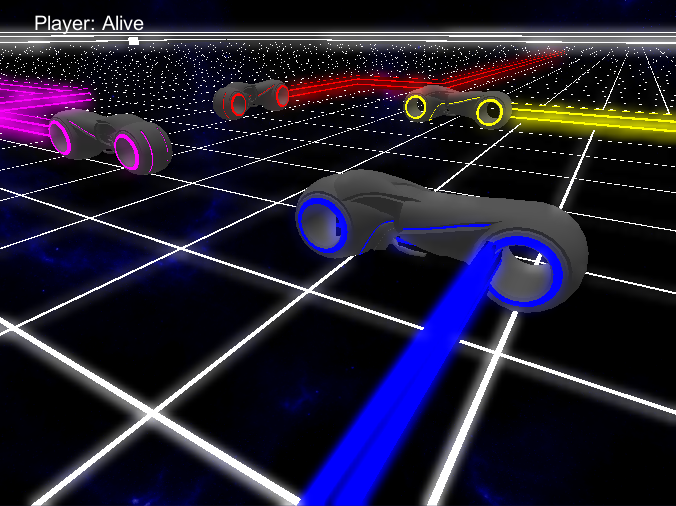
\includegraphics[height=6cm]{tron_four}
 	  
 	 	\caption{The main game... << weird wall >> }
 \end{figure}
 
\section{Gameplay and game mechanics }
We simplified AA to a single game mode, with fixed speed, arena size, etc.
We did, however, also extend the game to new concepts not present in any of the other versions. Specifically, we introduced collectible powerups and moving obstacles that roam the arena.

\begin{enumerate}
  \item you drive around in an arena
  \item the bike moves constantly and you can steer only by turning left or right at 90\textdegree \ angles.
  \item you leave a solid trail that is like a wall (and will be referred to as wall from now on)
  \item colliding with your own or another player's wall results in your death
  \item the aim is to be the last player alive
  \item being close to another wall increases your speed, allowing you to e.g. overtake other players.
  \item There are two different types of "power ups", which are randomly spawned items that will either increase your speed or make you invincible (you will be able to go through walls) for a short amount of time
  \item there are (optional?) obstacles in the form of large cubes that slowly "roll" around the arena, collisions with these also result in death.
 
\end{enumerate}


\section{Unity}
Unity, which is developed by Unity Technologies, is a relatively new game engine that is designed "to make game dev more democratic" >>find cit<<.
Unity includes the core engine which is used through an IDE that offers an editor >>fig<< that allows manipulation of 3D environments, game assets and live debugging.
Unity is based on Mono (an open source .NET-compatible framework) and allows development in JavaScript, Boo or C\#. 
We chose to use C\# because of its similarities to Java and Unity's integration with the extremely powerful Visual Studio IDE.
Unity supports a large number of plattforms, including x86/x86\_64 (Windows, Mac OS and Linux), Android, iOS and Windows Phone 8, with a generally very small required effort for porting between platforms.
The support for native x86 versions greately reduced the time needed for testing and debugging during development.

Unity's core concept is that of a "scene" which is an abstraction of a 3D space that contains "GameObjects".
"GameObjects" are containers that contain "Components" (which can also be GameObjects, allowing for nesting).
>>containers containing containers contained in ...<<
All "GO"s have a basic "transform" "component" which contains information about position, rotation and velocity of the "GO". There are many other types of components, including "Lights", "Cameras" and "Materials" as well as Scripts.

Unity offers two very different methods for networking.
A high-level "synchronization" feature as well as comparatively "low level"  Remote Procedure Calls (RPC).
Both require a GO to have a "NetworkView" component which makes them visible to the network in Unity.

Synchronization allows for high-frequency, low-cost updates  of GOs. It can however only be used to synchronize certain properties of the GO, e.g. the transform (pos,rot,vel) component.

RPC on the other hand, is intended to be used for less frequent and less time-sensitive communication and is very similar to RPC implementations in other frameworks.

\section{Networky stuff (ours)}
Our game combines (as >> will << most Unity applications) both methods, using Synchronization for player and wall positions (or more correctly player and wall "transforms"), as well as RPC for communicating gamestate changes.

In terms of networked multiplayer, most games can be classified into either an authorative or non-authorative server style.

With a non-authorative server, clients will do their own calculations locally and based on those will report e.g. their player's new position and events like the player's death to the server (and potentially other players). This is in contrast to an authorative server, where the client is mostly reduced to relaying the users input to the server which in turn does the necessary calculations and sends back information about   e.g. the player's position and liveness back to the clients.

Authorative servers have the advantage of preventing many common forms of cheating that involve running modified client code, however they also require a more powerful machine as server and result in additional latency.

Since our game is quite fast paced and supposed to run on relatively low-power mobile devices and will most likely not be subject to complicated cheating attempts, we feel that non-authorative server was the best fit for our application.


Updates regarding the movement of the player and the creation of new walls in a player's trail are handled by the player instance and are communicated using Unity's "state synchronization" system. 
The system offers two options for data transfer. One is a unity-specific reliable data protocol that uses delta compression (i.e. sending only the information that has changed) and ensures in-order delivery. The other is unreliable transmission via UDP.
Since in a racing game low latency is more important than in order-delivery, we use the UDP transmission mode.
<<is there anything else that we can say about this?>>

Spawning of new GameObjects (e.g. walls) is done via Unity's Network.Instantiate method, which automatically creates the same object on all clients.

Less frequent updates like e.g. player deaths and game start/end are sent via RPC.

Their is an "empty" (i.e. code-only) GameObject that contains the "MainController" which is responsible for updating the GUI and communicating (locally) state changes between the Game and the NetworkController.

The NetworkController causes events (via delegates) to be triggered in the MainController, which will then in turn call methods of the NetworkController or GameController.
The NetworkController handles all RPC. A received RPC will result in an event being triggered in MainController.
The MainController calls (non-RPC) functions of the NetworkController which will then in turn send out RPC Calls <<ATM machine?>> to the network.
Usually, RPC's will also be sent to the sender, ensuring that all clients make the same state transitions.

Since unity does not have a high-level concept representing the current application instance in its entirety, every script has to be attached to a GameObject and each instance (client?) will execute the same code for a given GameObject. 
Since our server instance will also be acting as a player/client instance, this model works well with our application design.

Checks like "Network.isMine()" or "Network.isServer()" allow to test wether the current GameObject (or more specifically its NetworkView) is owned by the current instance and whether we are acting as the server, respectively. 
<<move Since unity... back to beginning?>>

\section{Collisons/Powerups/Prediction}
If (drove into wall) \{
	players the Died 
	\}
	<< << >> >>

\section{ Opponents: AI + cubes}
In local singleplayer, there 
wenn KI stirbt hat sie 99% wkeit dass sie nochmal dreht.
50/50 links/rechts.

Nur jedes 2te frame darf sie sich drehen (sonst geht es auf der stelle)

0.005% links  0.000% rechts in jedem frame

Sch... simple aber effektiv.
<< >>


\section{Conclusion}
 Working in a larger group was an interesting change and while our intra team communication was good there were considerable efficiency losses when e.g. bugfixes for one component affected code that was concurrently being refactored.

 Wir glauben dass wir unser goal eine enjoyable networked multiplayer version zu builden gut erfüllt haben. Unity allowed us to very quickly create the visual aspects of the game and allowed <<doppel allowed>> us to focus on the distributed networking component of the game.

Eine naheliegender next step would be allowing the  player to customize the parameters of the game. Another interessante extension wäre Internet multiplayer,however additional work for NAT and higher latencies might be necessary.
\balancecolumns % GM June 2007

% The following two commands are all you need in the
% initial runs of your .tex file to
% produce the bibliography for the citations in your paper.
\bibliographystyle{abbrv}
\bibliography{report}  % sigproc.bib is the name of the Bibliography in this case
% You must have a proper ".bib" file


\end{document}
